\documentclass[sigconf,nonacm,pbalance]{acmart}
\usepackage{booktabs}
\usepackage{multirow}
\definecolor{hlred}{RGB}{196, 18, 28}
\newcommand{\hl}[1]{\textcolor{hlred}{\mathbf{#1}}}
\newcommand{\hlt}[1]{\textcolor{hlred}{\textbf{#1}}}
\emergencystretch=1.2em

\AtBeginDocument{%
  \providecommand\BibTeX{{%
    Bib\TeX}}}

\settopmatter{printacmref=false}

\raggedbottom
\clubpenalty=0
\widowpenalty=0
\begin{document}
\pagestyle{fancy}
\fancyhead{}
\fancyhead[L]{Preprint}
\fancyhead[R]{Overcoming Template Mega Clusters and Pooling Cancellation}

\title[Overcoming Template Mega Clusters and Pooling Cancellation]{Overcoming Template Mega Clusters and Pooling Cancellation in Unsupervised Incident Triage}
\subtitle{Preprint}

\author{Zakaria Sherif, Nicholas Cosereanu, and Wyatt Barker}
\affiliation{%
  \department{College of Computing and Software Engineering (CCSE)}
  \institution{Kennesaw State University}
  \country{}
}
\email{{zsherif, ncoserea, wbarker8}@students.kennesaw.edu}

\renewcommand{\shortauthors}{Sherif, Cosereanu, and Barker}

\begin{abstract}
Enterprise helpdesks and software repositories receive thousands of unstructured incident reports each quarter, and operations teams need to know which tickets belong together and which problems are growing. In our enterprise Information Technology Service Management (ITSM) benchmark, nearly one in four tickets (314 of 1,380 records) sit orphaned in an \texttt{Unassigned} backlog without a resolution timestamp because front line Tier 1 intake agents cannot determine which specialist team owns cross boundary security, network, or identity outages. Meanwhile, open source maintainers struggle to distinguish genuine user bug outbreaks from internal refactoring pull requests (PRs). We show that standard unsupervised topic modeling falls into two traps on these streams. In the \textbf{Template and Mega Cluster Trap}, automated word coherence metrics reward models that group recurring ticket boilerplate, while default density clustering merges distinct software bugs into one mega cluster. In the \textbf{Static Window Trap}, comparing two fixed periods suffers from \emph{pooling cancellation} (a drop in one month and a rise in the next cancel out once the months are combined) and cannot tell a short internal coding sprint from a chronic bug plateau. We present a three stage framework that avoids both traps: domain pruned term weighting with size bounded hierarchical density clustering (\textbf{Bounded EOM}) for discovery, false discovery rate (FDR) tests with 14 day rolling windows for shift tracking, and a check against withheld operational metadata. On open source GitHub issues and enterprise service desk tickets, the framework splits a 298 ticket mega cluster into five actionable subsystems, reveals four enterprise shifts that coarse windows erased, separates internal maintainer sprints from external user bug outbreaks, and groups 75.5\% of orphaned enterprise incidents with similar tickets that a team already handled.
\end{abstract}

\begin{CCSXML}
<ccs2012>
 <concept>
  <concept_id>10010147.10010178.10010179</concept_id>
  <concept_desc>Computing methodologies~Natural language processing</concept_desc>
  <concept_significance>500</concept_significance>
 </concept>
 <concept>
  <concept_id>10010147.10010257.10010258.10010260</concept_id>
  <concept_desc>Computing methodologies~Unsupervised learning</concept_desc>
  <concept_significance>500</concept_significance>
 </concept>
 <concept>
  <concept_id>10011007.10011074.10011111.10011696</concept_id>
  <concept_desc>Software and its engineering~Maintaining software</concept_desc>
  <concept_significance>300</concept_significance>
 </concept>
</ccs2012>
\end{CCSXML}

\ccsdesc[500]{Computing methodologies~Natural language processing}
\ccsdesc[500]{Computing methodologies~Unsupervised learning}
\ccsdesc[300]{Software and its engineering~Maintaining software}

\keywords{Incident Management, Topic Discovery, Density Clustering, Manifold Learning, Temporal Shift Detection, Site Reliability Engineering, Service Desk Triage}

\maketitle

\section{Introduction}
In enterprise Information Technology Service Management (ITSM), incoming support contacts are triaged through a tiered queue hierarchy~\cite{agarwal2012identifying, vogel2024itsm}: front line \emph{Tier 1} intake agents handle routine fulfillment requests and initial categorization, escalating unresolved technical faults to general \emph{Tier 2} support technicians or specialized engineering queues (such as network operations, endpoint security, or identity management). While routine requests (such as provisioning a software license or scheduling training) map cleanly to deterministic fulfillment workflows, complex infrastructure outages often produce ambiguous user symptoms that mask the underlying subsystem~\cite{chen2020incidental}. When a Tier 1 agent cannot identify the owning specialist department, tickets bounce across repeated queue reassignments or stagnate in generic holding queues. In a synthetic enterprise helpdesk benchmark~\cite{vogel2024itsm}, this diagnostic ambiguity leaves 314 error incidents (nearly one quarter of all incoming volume, almost half of them high or critical priority) completely orphaned in an \texttt{Unassigned} backlog without a recorded resolution. A parallel triage challenge arises in open source Site Reliability Engineering (SRE) and software maintenance~\cite{lhoest2021datasets, he2017drain}, where maintainers ingest a mixed stream of external user bug reports and internal developer pull requests (PRs) and must rapidly isolate postrelease regressions from routine refactoring~\cite{chen2020incidental}.

\begin{figure*}[t]
  \centering
  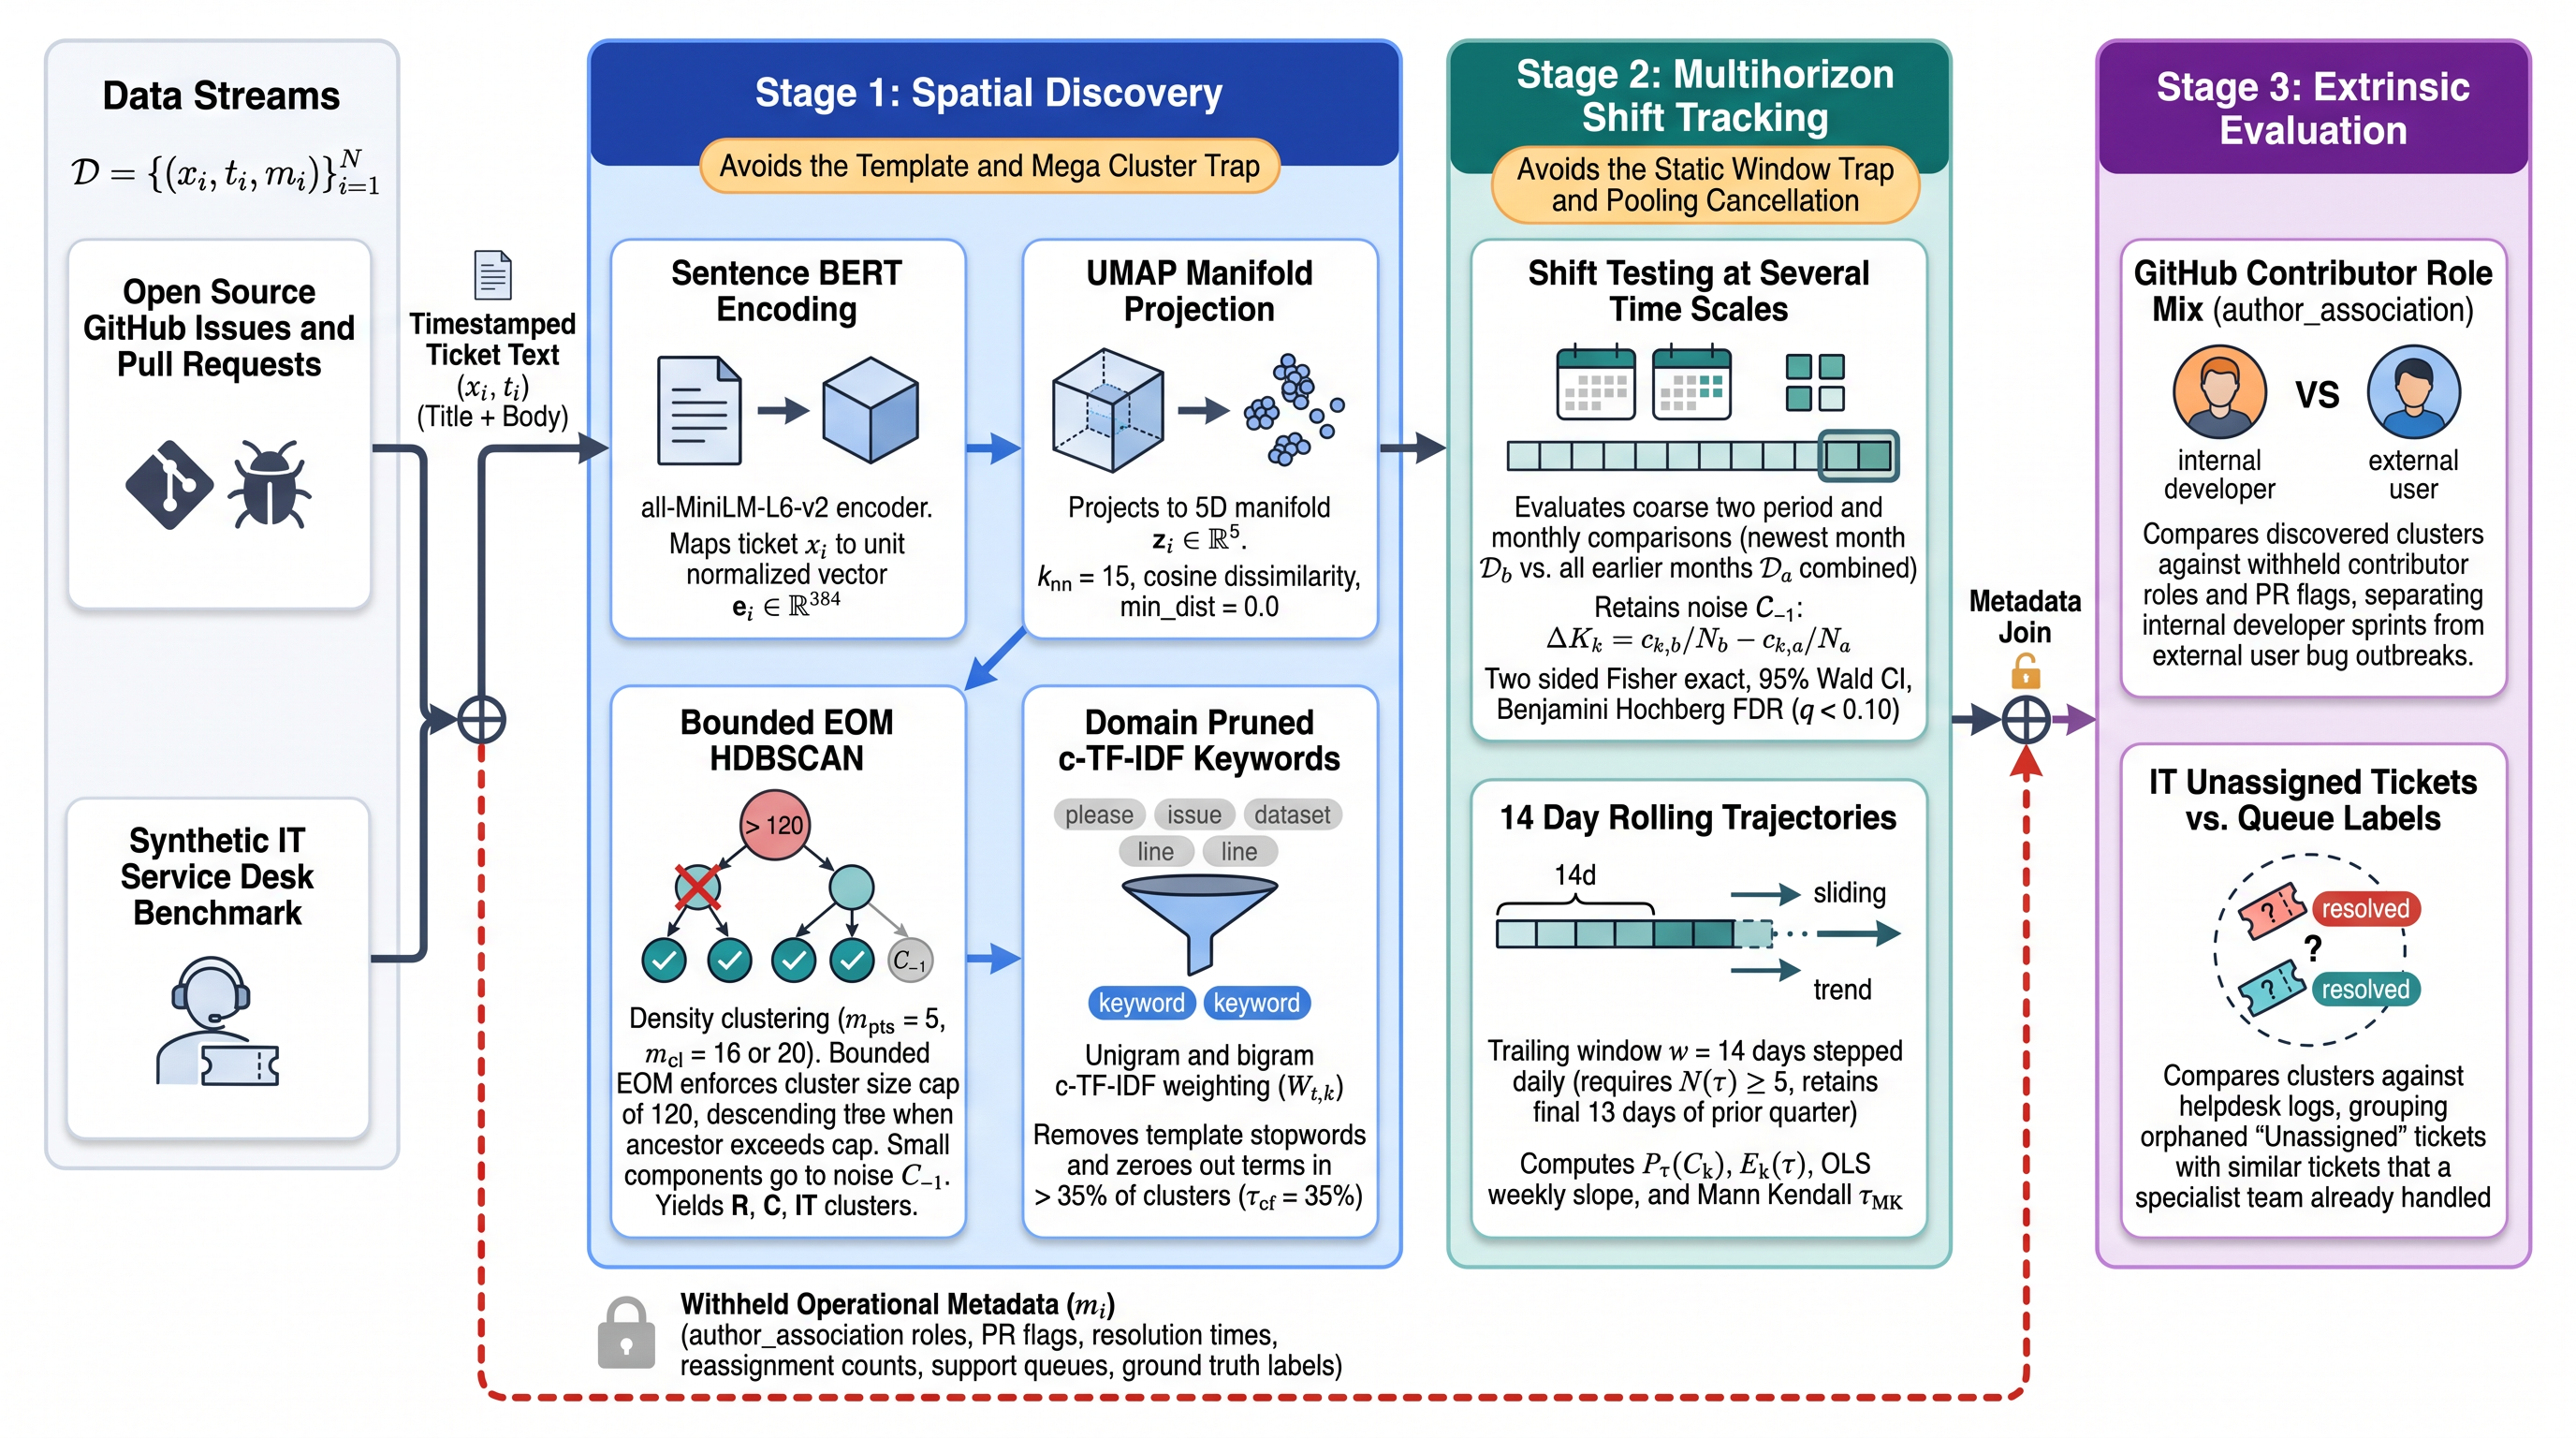
\includegraphics[width=0.96\textwidth]{figures/v6_figure1_architecture.png}
  \caption{Three Stage Incident Discovery, Shift Tracking, and Validation Pipeline}
  \label{fig:pipeline}
  \Description{Four column architecture diagram: two input corpora (open source GitHub issues and pull requests, and a synthetic IT service desk benchmark) feed Stage 1 (Sentence BERT encoding, UMAP projection to 5D, Bounded EOM HDBSCAN, domain pruned c-TF-IDF keywords), Stage 2 (shift testing at several time scales, and 14 day rolling trajectories), and Stage 3 (a GitHub contributor role view and an IT unassigned ticket versus queue label view). Withheld operational metadata follows a dashed path around Stages 1 and 2 and joins only before Stage 3.}
\end{figure*}

Unsupervised topic discovery~\cite{blei2003latent, grootendorst2022bertopic, dieng2020dynamic} offers a natural path to automate both intake routing and outbreak surveillance without requiring labeled training histories. By grouping semantically related tickets into clusters and tracking each cluster's prevalence over time, an operations team should be able to dispatch unassigned tickets to specialist queues and detect emerging failure surges as they form. Yet when practitioners apply standard topic modeling and drift monitoring pipelines to technical ticket streams, they encounter two systematic failure modes.

First, standard clustering pipelines fall into the \textbf{Template and Mega Cluster Trap}. Nearly every support ticket or bug issue contains recurring submission scaffolding such as \texttt{hello team}, \texttt{error message}, or \texttt{dataset, python, line}. Classical bag of words models such as Latent Dirichlet Allocation (LDA)~\cite{blei2003latent} group documents around these high frequency template words. Because template tokens cooccur across almost every sliding window in the corpus, LDA achieves deceptively high automated word coherence scores ($C_v$)~\cite{newman2010automatic, roder2015exploring} while mixing unrelated technical subsystems into the same topic~\cite{hoyle2021automated}. Neural pipelines following the BERTopic paradigm~\cite{grootendorst2022bertopic}, which encode text with Sentence-BERT (SBERT) transformers~\cite{reimers2019sentence, wang2020minilm}, project embeddings via Uniform Manifold Approximation and Projection (UMAP)~\cite{mcinnes2018umap}, and extract dense clusters via Hierarchical Density Based Spatial Clustering of Applications with Noise (HDBSCAN)~\cite{campello2013density, mcinnes2017hdbscan}, overcome lexical sparsity~\cite{sia2020tired, bianchi2021pre}. However, when distinct software failure modes share low level stack trace vocabulary (such as \texttt{pickle}, \texttt{dtype}, and \texttt{arrow}), HDBSCAN's default Excess of Mass (EOM) tree selection~\cite{campello2013density} overmerges them into a single ancestor ``mega cluster'' that obscures which specific subsystem is failing.

Second, standard temporal monitors fall into the \textbf{Static Window Trap}. Drift studies commonly partition a ticket stream into two static eras (a baseline window and an observation window) and rank topics by their proportional shift~\cite{chen2020incidental, dieng2020dynamic, grootendorst2022bertopic}. When a topic dips in one month and surges in the next, and both months fall inside the same observation window, the dip and the surge cancel out once the window is pooled. We call this \textbf{pooling cancellation}: the pooled share looks unchanged, hiding a major workload shift. Conversely, when a positive two period surge is detected, static windowing cannot tell whether the shift reflects a chronic bug plateau that persisted all quarter or a short internal coding sprint that already resolved.

We overcome both traps through the three stage framework illustrated in Figure~\ref{fig:pipeline} and evaluate it on open source software engineering issues~\cite{lhoest2021datasets} and enterprise IT service desk tickets~\cite{vogel2024itsm}. Specifically, we: (1) explain and resolve the coherence mirage and mega cluster overmerging using domain pruned term weighting and size bounded HDBSCAN tree selection (\textbf{Bounded EOM}); (2) pair Benjamini--Hochberg false discovery rate (FDR) contingency testing~\cite{fisher1922interpretation, benjamini1995controlling} with continuous 14 day rolling trajectories~\cite{mann1945nonparametric, kendall1948rank} to expose shifts hidden by pooling cancellation and separate chronic plateaus from transient spikes; and (3) validate our clusters against withheld contributor roles and helpdesk routing logs, separating internal developer sprints from external user bug outbreaks and grouping orphaned enterprise incidents with similar tickets that a team already handled.

\section{Related Work}
Generative topic models such as LDA~\cite{blei2003latent} and Dynamic Embedded Topic Models (DETM)~\cite{dieng2020dynamic} represent documents as mixtures over word distributions, whereas modular neural pipelines decouple dense representation learning from keyword extraction~\cite{sia2020tired, bianchi2021pre, grootendorst2022bertopic}. Following BERTopic~\cite{grootendorst2022bertopic}, embedding pipelines pair transformer encoders~\cite{reimers2019sentence, wang2020minilm}, UMAP projection~\cite{mcinnes2018umap}, HDBSCAN clustering~\cite{campello2013density, mcinnes2017hdbscan}, and c-TF-IDF weighting. More recently, prompt based frameworks such as TopicGPT~\cite{pham2024topicgpt} query large language models (LLMs) directly to induce topic labels. However, transmitting raw helpdesk tickets to external LLM APIs raises enterprise data privacy barriers, incurs high per ticket inference cost at intake scale, and risks taxonomy drift across batches. Meanwhile, Hoyle et al.~\cite{hoyle2021automated} showed that sliding window coherence metrics~\cite{newman2010automatic, roder2015exploring} correlate poorly with human judgment on general text; we pinpoint why templated tickets invert coherence rankings and bound HDBSCAN tree selection so local density clustering avoids parent mega clusters.

In software engineering and service desk automation, prior work spans syntax tree log parsers such as Drain~\cite{he2017drain}, supervised developer and queue routers~\cite{anvik2006who, agarwal2012identifying, chen2020incidental}, and fine tuned or prompted LLMs that recommend cloud root causes and mitigations from historical postmortems~\cite{ahmed2023recommending}. Supervised classifiers and fine tuned LLMs depend on labeled routing histories, faltering when novel postrelease regressions emerge or when front line intake leaves cross boundary tickets \texttt{Unassigned}~\cite{chen2020incidental}. Our unsupervised approach groups unlabeled tickets strictly by failure text and uses resolved neighbors only post hoc to infer owning queues.

Finally, classical burst models~\cite{kleinberg2002bursty} and concept drift detectors~\cite{gama2014survey} track distributional shifts in evolving streams, whereas dynamic topic pipelines typically bin cluster counts into fixed calendar intervals~\cite{dieng2020dynamic, grootendorst2022bertopic}. On incident streams, uncalibrated bin differences inflate false alarms across dozens of clusters while static two period splits suffer from pooling cancellation. Section~\ref{sec:method} pairs FDR controlled contingency testing with continuous rolling trend estimation to address both failure modes.

\section{Methodology}
\label{sec:method}

\subsection{Overview and Problem Formulation}
Our pipeline processes each ticket through three stages (Figure~\ref{fig:pipeline}). Stage 1 embeds ticket text, projects similar tickets onto a low dimensional manifold, and extracts size bounded clusters representing single failure modes. Stage 2 tests cluster count shifts against chance across both two period splits and 14 day rolling windows. Stage 3 validates clusters against unseen operational records such as contributor roles and handling teams. Throughout, \texttt{R} clusters denote unconstrained (standard EOM) HDBSCAN clusters on GitHub, \texttt{C} clusters denote Bounded EOM GitHub clusters, and \texttt{IT} clusters denote enterprise service desk clusters.

Formally, the pipeline ingests a timestamped stream $\mathcal{D} = \{(x_i, t_i, m_i)\}_{i=1}^{N}$, where $x_i$ concatenates ticket title and body, $t_i$ is creation time, and $m_i$ denotes operational metadata (contributor roles, PR flags, resolution times, reassignment counts, and support queues). All metadata $m_i$ is withheld during Stages 1 and 2 and reserved for Stage 3 validation: resolution times and true owning queues do not exist at intake, text only clustering groups tickets by failure mechanism rather than noisy routing tags, and withholding $m_i$ prevents circular validation.

\subsection{Manifold Projection and Bounded Density Clustering}
Each ticket $x_i$ is mapped into a unit normalized vector $\mathbf{e}_i \in \mathbb{R}^{384}$ using the pretrained \texttt{all-MiniLM-L6-v2} Siamese Sentence-BERT encoder~\cite{reimers2019sentence, wang2020minilm}. Because cosine distances between distinct documents concentrate around their mean in high dimensional space~\cite{beyer1999nearest}, which erases the density valleys needed for spatial clustering, we project $\{\mathbf{e}_i\}_{i=1}^{N}$ onto a 5 dimensional manifold $\{\mathbf{z}_i\}_{i=1}^{N}$ via UMAP~\cite{mcinnes2018umap} using local neighborhood size $k_{\text{nn}} = 15$, cosine dissimilarity, and zero minimum packing distance ($\text{min\_dist} = 0.0$).

On the 5D manifold, we apply HDBSCAN~\cite{campello2013density, mcinnes2017hdbscan} with minimum sample size $m_{\text{pts}} = 5$ and minimum cluster size $m_{\text{cl}} = 16$ ($20$ on the larger enterprise IT corpus). To suppress sparse background noise, HDBSCAN defines the \emph{mutual reachability distance} between tickets $i$ and $j$ as the maximum of their $m_{\text{pts}}$ nearest neighbor core distances and their Euclidean distance, pushing isolated outliers away from dense regions. Constructing a minimum spanning tree over mutual reachability distances yields a condensed cluster tree across density levels $\lambda = 1 / \text{distance}$, where branches smaller than $m_{\text{cl}}$ fall into an explicit noise partition $C_{-1}$. Standard HDBSCAN extracts flat clusters from this condensed tree via Excess of Mass (EOM), selecting branches that maximize integrated density persistence:
\begin{equation}
\label{eq:eom}
S(C_k) = \sum_{x_i \in C_k} \left( \lambda_{\text{max}}(x_i, C_k) - \lambda_{\text{min}}(C_k) \right),
\end{equation}
where $\lambda_{\text{min}}(C_k)$ is the density level at which cluster $C_k$ splits from its parent and $\lambda_{\text{max}}(x_i, C_k)$ is the level at which ticket $x_i$ leaves $C_k$. When distinct technical subsystems share common stack trace tokens, their density branches merge at moderate reachability thresholds, causing unconstrained EOM in Equation~\ref{eq:eom} to select a single merged ancestor cluster. To prevent mega cluster absorption without incurring the severe outlier rejection of terminal leaf clustering, we introduce \textbf{Bounded EOM (BEOM)}, which caps maximum cluster size at $M_{\max} = \lceil \alpha N \rceil$ tickets ($\alpha \approx 0.14$, giving $120$ tickets on our $N = 881$ SWE stream so no single cluster absorbs more than $\sim\!14\%$ of workload) and traverses down the condensed tree to select descendant subsystem branches whenever an ancestor exceeds that cap. Expressing $M_{\max}$ as a workload share $\alpha N$ allows the cap to scale across smaller startups and high volume enterprises, though homogeneous high volume fulfillment queues may not need splitting (Section~\ref{sec:corpora}).

\subsection{Domain Pruned Class Based Term Weighting}
To extract human interpretable topic descriptors without generative word priors, we concatenate all documents assigned to cluster $C_k$ and compute class based TF-IDF (c-TF-IDF) weights~\cite{grootendorst2022bertopic} over unigrams and bigrams:
\begin{equation}
\label{eq:ctfidf}
W_{t, k} = \frac{f_{t, k}}{\sum_{t' \in \mathcal{V}} f_{t', k}} \cdot \left( \ln \left( \frac{K + 1}{\text{cf}_t + 1} \right) + 1 \right),
\end{equation}
where $\mathcal{V}$ is the candidate vocabulary, $f_{t, k}$ is the frequency of term $t$ in $C_k$, and $\text{cf}_t$ is the number of clusters containing $t$. Whereas our \textbf{Standard (\texttt{Std.})} setting removes only standard English stopwords, our \textbf{Domain Pruned (\texttt{Pruned})} filter~\cite{hoyle2021automated, bianchi2021pre, grootendorst2022bertopic} augments English stopwords with recurring ticket template tokens (e.g., \texttt{please}, \texttt{issue}, \texttt{dataset}, \texttt{line}) and zeroes out terms appearing in more than $\tau_{\text{cf}} = 35\%$ of discovered clusters ($40\%$ on IT) so top ranked keywords uniquely identify the underlying failure mode.

\subsection{Multihorizon Shift Testing and Rolling Trajectories}
Given a baseline partition $\mathcal{D}_a$ ($N_a$ tickets) and an observation partition $\mathcal{D}_b$ ($N_b$ tickets), we retain all valid timestamped records, including noise $C_{-1}$, in the denominator so cluster prevalence $P(C_k \mid \mathcal{D}) = c_k / N$ measures true share of total operational workload and $\Delta K_k$ tracks the shift in percentage points (pp):
\begin{equation}
\label{eq:deltak}
\Delta K_k = P(C_k \mid \mathcal{D}_b) - P(C_k \mid \mathcal{D}_a) = \frac{c_{k, b}}{N_b} - \frac{c_{k, a}}{N_a}.
\end{equation}
We test each cluster's $2 \times 2$ contingency table with a two sided Fisher's exact test~\cite{fisher1922interpretation}, compute 95\% Wald confidence intervals for the proportion difference, and control familywise false discovery rate (FDR) across all $K$ clusters via Benjamini--Hochberg (BH) adjusted $q$ values ($q < 0.10$)~\cite{benjamini1995controlling}. To avoid pooling cancellation, we run both a coarse two period test and a monthly test comparing each new month $\mathcal{D}_b$ against all prior months $\mathcal{D}_a$ combined.

To capture subperiod dynamics erased by two window splits, we slide a trailing $w = 14$ day window $\mathcal{W}(\tau) = (\tau - w, \tau]$ daily across the stream, retaining the prior quarter's final $w - 1$ days for boundary continuity. Across $w \in \{7, 14, 21, 28\}$ days on our streams ($\sim\!5$ to $15$ tickets/day), $w = 14$ spans two weekly work and sprint cycles, halving $7$ day jitter while avoiding the $5$ to $11$ day peak lag of $21$ and $28$ day windows; deployments at different scales should adjust $w$ inversely with arrival rate to preserve window sample support. At each day $\tau$ with $N(\tau) \ge 5$ tickets, we compute rolling prevalence $P_\tau(C_k) = c_k(\tau) / N(\tau)$, baseline excess $E_k(\tau) = P_\tau(C_k) - P(C_k \mid \mathcal{D}_{\text{base}})$, linear weekly slope (pp/wk), and the Mann--Kendall monotonic trend $\tau_{\text{MK}} \in [-1, 1]$~\cite{mann1945nonparametric, kendall1948rank}.


\begin{figure}[!htbp]
  \centering
  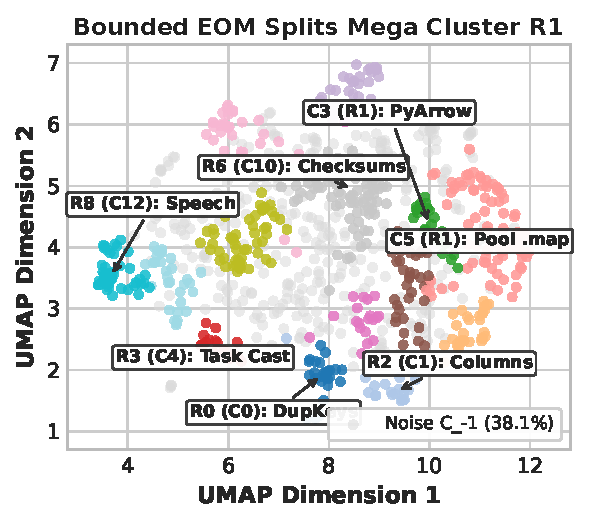
\includegraphics[width=0.85\linewidth]{figures/v4_figure2_r1_split.pdf}
  \caption{2D UMAP Projection of the GitHub Corpus Under Bounded EOM Clustering}
  \label{fig:spatial}
  \Description{2D UMAP scatter plot of 881 GitHub issues and pull requests colored by the 14 Bounded EOM clusters (C0 through C13), with gray points indicating unclustered HDBSCAN noise. Callout labels show that the overmerged standard EOM cluster R1 splits into five spatially distinct subsystem clusters (C2 tensor casting, C3 PyArrow ABI, C5 multiprocessing pickle, C7 Arrow disk index, and C8 tokenizer bindings), whereas the remaining nine clusters (R0 and R2 through R9) map one to one to single Bounded EOM clusters.}
\end{figure}

\section{Experimental Setup}

\subsection{Benchmark Corpora}
\label{sec:corpora}
To evaluate generalization across distinct operational environments, we test our framework on two timestamped corpora (Figure~\ref{fig:pipeline}). First, the open source software engineering (SWE) corpus from the Hugging Face \texttt{datasets} GitHub repository~\cite{lhoest2021datasets} comprises $N = 881$ records across Q1 2021 ($478$ records) and Q2 2021 ($403$ records), pairing issue ($41.7\%$) and pull request ($58.3\%$) text with withheld GitHub \texttt{author\_association} roles (\texttt{MEMBER}, \texttt{CONTRIBUTOR}, or external community user \texttt{NONE}), maintainer tags, and Mean Time to Resolution (MTTR, elapsed hours from opening to closure). Second, the enterprise IT service desk benchmark~\cite{vogel2024itsm}, a publicly released synthetic dataset of IT call center tickets, contains $N = 1,380$ records spanning Q1 2021 ($1,338$ tickets across January, February, and March) plus a multiyear 2024 slice ($42$ tickets), with curated ground truth labels for ticket type (\texttt{Incident} versus \texttt{Request}), category, subcategory, priority, reassignment count (queue hops), 15 specialist support queues, and $314$ unassigned Q1 error incidents. On this corpus, the model benchmark in Table~\ref{tab:exp1} compares both standard EOM ($K = 14$) and Bounded EOM ($K = 22$). Because the IT stream has no mixed mega cluster under standard EOM (its largest cluster is a single homogeneous software installation queue, and the five critical outage families already reach $93.8\%$ to $100\%$ subcategory purity), the shift analysis (Section~\ref{sec:itshift}) and the triage evaluation (Section~\ref{sec:ittriage}) use the standard EOM clusters ($m_{\text{cl}} = 20$, $m_{\text{pts}} = 6$, labeled \texttt{IT00} to \texttt{IT13}) to retain higher ticket coverage ($14.9\%$ noise versus $34.5\%$ under Bounded EOM, where the 120 ticket cap subdivides large routine queues).

\subsection{Baselines and Metric Interpretation}
Unlike parametric models, HDBSCAN determines the non noise cluster count $K$ automatically from the density tree: on SWE, standard EOM discovers $K = 10$ (\texttt{R0} to \texttt{R9}) and Bounded EOM discovers $K = 14$ (\texttt{C0} to \texttt{C13}); on IT, standard EOM discovers $K = 14$ (\texttt{IT00} to \texttt{IT13}) and Bounded EOM discovers $K = 22$. Rather than tuning $K$ to favor any method, we evaluate three parametric baselines at matching cluster counts ($K = 10$ and $14$): classical generative LDA~\cite{blei2003latent}, sparse TF-IDF with $K$ Means (TF-IDF+KM), and dense 384D Sentence-BERT embeddings with $K$ Means (SBERT+KM)~\cite{reimers2019sentence}. In Table~\ref{tab:exp1}, the top two SWE blocks isolate the stopword ablation (\texttt{Std.} versus \texttt{Pruned}, Section~\ref{sec:method}), while the bottom IT block evaluates cross domain purity under \texttt{Pruned}.

To aid interpretation across Tables~\ref{tab:exp1} to~\ref{tab:exp8}, each metric captures a distinct property: (1) \textbf{Noise} ($\%$) is the share of ambiguous outliers placed in $C_{-1}$ ($0\%$ for forced $K$ Means/LDA partitions); (2) \textbf{$C_v$ Coherence} ($\in [0, 1]$)~\cite{newman2010automatic, roder2015exploring} averages sliding window ($110$ tokens, stride $25$) Normalized Pointwise Mutual Information (NPMI) context similarity among top words (normally higher is better, \emph{except} recurring ticket templates artificially inflate it); (3) \textbf{Topic Diversity} (\textbf{Div.} $\in [0, 1]$, higher $\uparrow$ is better) is the unique fraction among the top 10 words across all $K$ clusters ($1.00$ means zero keyword overlap); (4) \textbf{Silhouette} (\textbf{Sil.384}, \textbf{Sil.5D} $\in [-1, 1]$, higher $\uparrow$ is better)~\cite{rousseeuw1987silhouettes} measures within cluster cohesion versus nearest cluster separation over assigned tickets ($>0$ well separated, $<0$ overlapping); (5) \textbf{IT Type / Sub. Purity} ($\%$, higher $\uparrow$ is better) is the share of assigned IT tickets matching their cluster's majority ground truth \texttt{Incident}/\texttt{Request} type or fine subcategory; and (6) in Tables~\ref{tab:exp2} and~\ref{tab:exp8}, \textbf{$\Delta K$} (percentage points, pp) is the workload share shift between periods, \textbf{$q$} ($\in [0, 1]$, significant at $q < 0.10$) is the BH FDR adjusted Fisher $p$ value, and \textbf{$\tau_{\text{MK}}$} ($\in [-1, 1]$) is the 14 day rolling monotonic trend ($>0$ rising, $<0$ falling, $\approx 0$ flat plateau or up and down spike).

\section{Overcoming Trap 1: The Template Coherence Mirage and Mega Clusters}

\subsection{Why High Word Coherence Is a Mirage on Ticket Streams}
Across both operational benchmarks, Table~\ref{tab:exp1} reveals an inverse relationship between bag of words coherence and geometric or operational validity. Lexical bag of words baselines achieve the highest $C_v$ coherence across all blocks of Table~\ref{tab:exp1}, led by classical LDA on SWE ($0.948$ standard; $0.910$ pruned) and by sparse TF-IDF+$K$ Means ($0.937$) followed by LDA ($0.905$) on IT, yet both baselines suffer negative or near zero 5D manifold Silhouette scores ($-0.225$ to $0.058$) while LDA ranks last on every enterprise ground truth metric.

\begin{table}[!htbp]
  \caption{Topic Modeling and Clustering Benchmark Across Both Operational Streams}
  \label{tab:exp1}
  \footnotesize
  \setlength{\tabcolsep}{1.35pt}
  \begin{tabular}{llrrrrrr}
    \toprule
    Stream / Filter & Model ($K$) & Noise & $C_v$ & Div.$\uparrow$ & Sil.384$\uparrow$ & Sil.5D$\uparrow$ & IT Type / Sub.$\uparrow$ \\
    \midrule
    SWE / Std. & LDA (10) & 0.0\% & .948 & .670 & $-.032$ & $-.108$ & n/a \\
    SWE / Std. & TF-IDF+KM (10) & 0.0\% & .882 & .810 & $-.026$ & $-.168$ & n/a \\
    SWE / Std. & SBERT+KM (10) & 0.0\% & .853 & .760 & $.026$ & $.043$ & n/a \\
    SWE / Std. & BEOM (14) & 38.1\% & .862 & .800 & $\hl{.051}$ & $\hl{.531}$ & n/a \\
    \addlinespace[2pt]
    SWE / Pruned & LDA (14) & 0.0\% & .910 & .807 & $-.035$ & $-.225$ & n/a \\
    SWE / Pruned & TF-IDF+KM (14) & 0.0\% & .718 & 1.00 & $-.034$ & $-.194$ & n/a \\
    SWE / Pruned & SBERT+KM (14) & 0.0\% & .654 & .943 & $.030$ & $.059$ & n/a \\
    SWE / Pruned & EOM (10) & 27.2\% & .691 & $\hl{.960}$ & $.026$ & $.378$ & n/a \\
    SWE / Pruned & BEOM (14) & 38.1\% & .694 & $\hl{.943}$ & $\hl{.051}$ & $\hl{.531}$ & n/a \\
    \addlinespace[2pt]
    IT / Pruned & LDA (14) & 0.0\% & .905 & .836 & $.021$ & $-.060$ & 85.5 / 63.6\% \\
    IT / Pruned & TF-IDF+KM (14) & 0.0\% & .937 & .900 & $.039$ & $.058$ & 92.6 / 80.4\% \\
    IT / Pruned & SBERT+KM (14) & 0.0\% & .874 & .936 & $.083$ & $.269$ & 95.5 / 78.6\% \\
    IT / Pruned & EOM (14) & 14.9\% & .840 & $\hl{.979}$ & $\hl{.100}$ & $\hl{.559}$ & 96.6 / 76.0\% \\
    IT / Pruned & BEOM (22) & 34.5\% & .897 & .914 & $\hl{.092}$ & $\hl{.588}$ & $\hlt{98.3}$ / $\hlt{82.3\%}$ \\
    \bottomrule
  \end{tabular}
\end{table}

This paradox arises from how sliding window NPMI evaluates word cooccurrence in templated text~\cite{hoyle2021automated}. Because submission boilerplate (\texttt{dataset}, \texttt{github}, \texttt{python}, \texttt{error message}) appears in nearly every ticket, LDA places slight permutations of these ubiquitous tokens at the top of multiple topics, depressing Topic Diversity ($0.670$). Because boilerplate words cooccur across almost every 110 token window, their pairwise NPMI is artificially inflated, rewarding LDA with a high $C_v$ score even though documents sharing template words describe unrelated technical failures and scatter across the embedding space.

Stripping domain boilerplate (middle and bottom blocks of Table~\ref{tab:exp1}) forces c-TF-IDF to rank subsystem specific identifiers (\texttt{duplicatedkeyserror}, \texttt{prepare\_for\_task}, \texttt{crowdstrike falcon}). Because specialized identifiers appear only within narrow failure modes, corpus wide window cooccurrence drops, lowering $C_v$ while lifting Topic Diversity above $0.94$. Crucially, comparing $K$ Means against Bounded EOM on the enterprise stream reveals why density clustering excels at fine grained triage: whereas forced $K$ Means partitioning assigns every ambiguous ticket to its nearest centroid and blurs fine subcategory boundaries, Bounded EOM quarantines cross cutting outliers into $C_{-1}$ to achieve the highest manifold separation alongside $98.3\%$ incident versus request purity and $82.3\%$ subcategory purity. Even when noise points are assigned to their nearest centroid to evaluate 100\% of the SWE corpus, our pipeline retains a sixfold advantage in 5D Silhouette over dense $K$ Means ($0.354$ versus $0.059$).

\subsection{Breaking the 298 Ticket Mega Cluster with Bounded EOM}
Manifold projection must precede density clustering: in raw 384D SBERT space, cosine distance concentration~\cite{beyer1999nearest} flattens density differences so severely that HDBSCAN rejects $98.2\%$ of the corpus as noise, whereas the 5D projection restores the dense regions that clusters need.

Within this 5D manifold, however, comparing unbounded EOM ($K = 10$, clusters \texttt{R0} to \texttt{R9}) against Bounded EOM ($K = 14$, clusters \texttt{C0} to \texttt{C13}, $\text{max\_cluster\_size} = 120$) exposes a critical hierarchical overmerging effect~\cite{campello2013density, lhoest2021datasets}. Left unconstrained, a single parent cluster (\texttt{R1}) absorbs $33.8\%$ of the entire GitHub corpus ($46.5\%$ of assigned records). Cross tabulating cluster memberships across the condensed tree reveals that Bounded EOM leaves the nine specialized clusters (\texttt{R0}, \texttt{R2} to \texttt{R9}) completely unchanged (Adjusted Rand Index~\cite{hubert1985comparing} $\text{ARI} = 1.000$ outside \texttt{R1}), while splitting the 298 ticket \texttt{R1} ancestor into five mechanically distinct subsystems in Figure~\ref{fig:spatial} and Table~\ref{tab:exp2}: multiprocessing worker pool \texttt{.map()} serialization (\texttt{pickle}) locks (\texttt{C5}, $N = 92$), Apache Arrow columnar \texttt{int64} memory mapped index collisions (\texttt{C7}, $N = 35$), PyArrow C++ Application Binary Interface (ABI) and Conda wheel conflicts (\texttt{C3}, $N = 23$), tensor format casting (\texttt{C2}, $N = 31$), and tokenizer C++ \texttt{\_libs} bindings (\texttt{C8}, $N = 21$). Because all five failure modes share low level stack trace tokens (\texttt{pickle}, \texttt{dtype}, \texttt{arrow}), their branches merge near the root of the condensed tree; enforcing the Bounded EOM size cap selects the descendant branches instead, cutting maximum cluster share nearly in thirds ($46.5\%$ to $16.9\%$). We now examine how their prevalence evolves across coarse and continuous time horizons.

\section{Overcoming Trap 2: The Static Window Trap}

\subsection{Unmixing the Mega Cluster and Separating Sprints from Chronic Bugs on GitHub}
Applying Fisher's exact tests~\cite{fisher1922interpretation} and Benjamini--Hochberg FDR control~\cite{benjamini1995controlling} to the unified GitHub hierarchy in Table~\ref{tab:exp2} demonstrates why hierarchical unmixing is essential for accurate drift attribution.

\begin{table}[!htbp]
  \caption{Quarterly Prevalence Shifts and Hierarchical Mega Cluster Unmixing on the GitHub Stream}
  \label{tab:exp2}
  \footnotesize
  \setlength{\tabcolsep}{1.15pt}
  \begin{tabular}{llrrrrr}
    \toprule
    ID & Subsystem & Q1 & Q2 & $\Delta K$ & $q$ & $\tau_{\text{MK}}$ ($p$) \\
    \midrule
    \texttt{R1} (EOM) & Serialization Parent & 30.3\% & 38.0\% & $\hl{+7.6}$ & $\hl{.046}$ & $+.01$ (.94) \\
    \hspace{2pt}$\hookrightarrow$\texttt{C5} & Pool \texttt{.map()} Pickle & 8.2\% & 13.2\% & $\hl{+5.0}$ & $\hl{.070}$ & $+.08$ (.27) \\
    \hspace{2pt}$\hookrightarrow$\texttt{C7} & Arrow Disk Index & 2.9\% & 5.2\% & $+2.3$ & $.201$ & $+.04$ (.58) \\
    \hspace{2pt}$\hookrightarrow$\texttt{C3} & PyArrow C++ ABI & 2.1\% & 3.2\% & $+1.1$ & $.381$ & $-.03$ (.69) \\
    \hspace{2pt}$\hookrightarrow$\texttt{C2} & Tensor / JAX Cast & 4.2\% & 2.7\% & $-1.5$ & $.381$ & $-.11$ (.13) \\
    \hspace{2pt}$\hookrightarrow$\texttt{C8} & Tokenizer \texttt{\_libs} & 3.1\% & 1.5\% & $-1.6$ & $.201$ & $-.14$ (.05) \\
    \addlinespace[2pt]
    \texttt{R3} (\texttt{C4}) & Task Prompt Cast & 0.4\% & 4.5\% & $\hl{+4.1}$ & $\hl{.001}$ & $\hl{+.36}$ (\hlt{1e-6}) \\
    \texttt{R0} (\texttt{C0}) & DuplicateKeys Hash & 1.7\% & 5.2\% & $\hl{+3.5}$ & $\hl{.019}$ & $+.10$ (.15) \\
    \texttt{R5} (\texttt{C9}) & Sphinx Docs Build & 2.9\% & 4.2\% & $+1.3$ & $.400$ & $+.00$ (.97) \\
    \texttt{R4} (\texttt{C6}) & CER / WER Metrics & 2.9\% & 3.7\% & $+0.8$ & $.572$ & $+.03$ (.65) \\
    \texttt{R2} (\texttt{C1}) & Table \texttt{rename\_col} & 2.7\% & 1.7\% & $-1.0$ & $.400$ & $-.58$ (1e-13) \\
    \texttt{R8} (\texttt{C12}) & Speech ASR Audio & 6.1\% & 3.7\% & $-2.3$ & $.201$ & $-.16$ (.03) \\
    \texttt{R9} (\texttt{C13}) & PDF / DuoRC Parse & 4.6\% & 2.2\% & $-2.4$ & $.187$ & $-.29$ (5e-5) \\
    \texttt{R7} (\texttt{C11}) & Hub Cards / C4 & 7.5\% & 5.0\% & $-2.6$ & $.201$ & $+.32$ (8e-6) \\
    \texttt{R6} (\texttt{C10}) & NumPy / Checksums & 12.6\% & 5.7\% & $\hl{-6.8}$ & $\hl{.003}$ & $-.16$ (.03) \\
    \bottomrule
  \end{tabular}
\end{table}

\begin{figure}[!htbp]
  \centering
  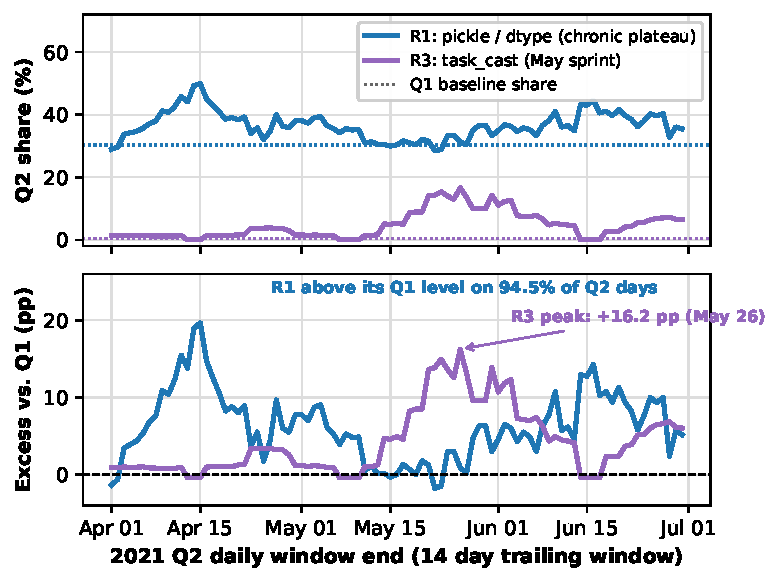
\includegraphics[width=0.88\linewidth]{figures/v3_figure3_r1_r3_rolling.pdf}
  \caption{14 Day Rolling Prevalence and Baseline Excess Trajectories for Clusters R1 and R3}
  \label{fig:q2excess}
  \Description{Two panel time series for clusters R1 and R3 only: the top panel shows 14 day trailing prevalence across Q2 2021 with dotted Q1 baseline lines, and the bottom panel shows percentage point excess relative to the Q1 baseline.}
\end{figure}

\begin{figure*}[t]
  \centering
  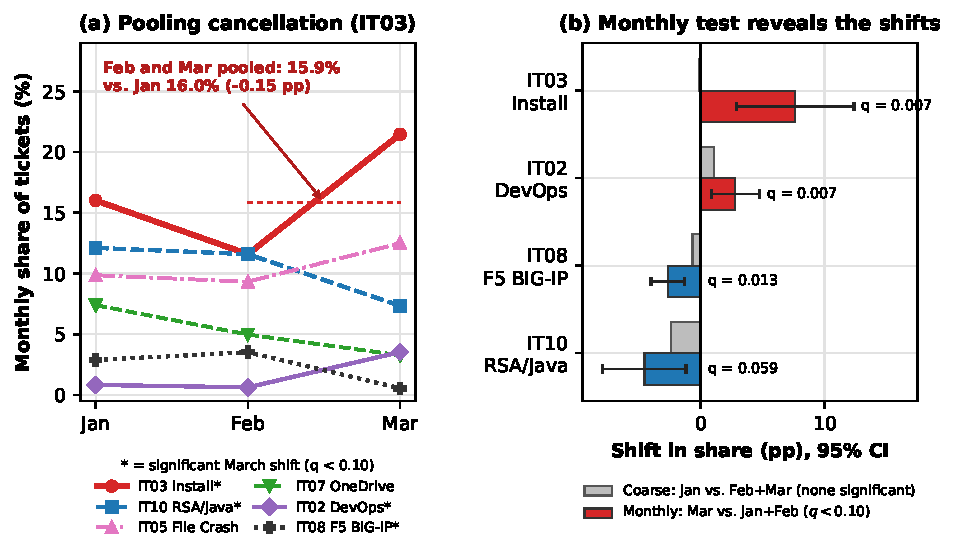
\includegraphics[width=0.80\textwidth]{figures/v4_figure4_pooling_cancellation.pdf}
  \caption{Monthly Topic Shares and Shift Confidence Intervals on the Enterprise IT Stream}
  \label{fig:temporal_sens}
  \Description{Two panel figure. Panel a is a line chart of monthly topic shares for six IT clusters across January, February, and March, with a dashed line showing IT03's pooled February and March share next to its January share. Panel b is a horizontal bar chart comparing the coarse shift and the monthly March shift with 95 percent confidence intervals for IT03, IT02, IT08, and IT10.}
\end{figure*}

Under unbounded EOM, the parent cluster \texttt{R1} appears to surge broadly across nearly two fifths of the repository. Bounded EOM decomposition in Table~\ref{tab:exp2} (where CER/WER denotes Character/Word Error Rate in \texttt{R4} and ASR denotes Automatic Speech Recognition in \texttt{R8}) proves that \textbf{only the multiprocessing \texttt{.map()} pickle branch (\texttt{C5}) experienced a statistically significant Q2 surge}, while the other four subbranches inside \texttt{R1} remained stationary or declined. The three significant Q2 surges are cross process \texttt{pickle} failures in parallel \texttt{.map()} workers (\texttt{C5}), shard key uniqueness errors (\texttt{R0}), and task template casting (\texttt{R3}), while remote downloader checksum failures (\texttt{R6}) declined significantly. Comparing \texttt{C7} ($+2.3$ pp, $q = 0.201$) against \texttt{R3} ($+4.1$ pp, $q = 0.001$) also shows why uncalibrated point cutoffs fail: because binomial variance scales with baseline share $p(1-p)$, a $+4.1$ pp jump from a $0.4\%$ baseline represents an $11\times$ outbreak, whereas a $+2.3$ pp fluctuation atop a $2.9\%$ baseline lies within expected quarterly variation.

Even when statistically calibrated, coarse two period deltas obscure the within quarter shape of a shift. Tracking continuous 14 day rolling windows across all 91 days of Q2 in Figure~\ref{fig:q2excess} and the $\tau_{\text{MK}}$ column of Table~\ref{tab:exp2} reveals that \texttt{R1} and \texttt{R3} follow opposite temporal regimes despite both registering positive quarterly surges. Serialization failures in \texttt{R1} jump at the start of April and remain chronically elevated above their Q1 baseline on $94.5\%$ of Q2 days (mean excess $+6.29$ pp); because this step change plateaued early in the quarter, its within quarter linear slope ($-0.06$ pp/wk) and Mann--Kendall trend $\tau_{\text{MK}}$~\cite{mann1945nonparametric, kendall1948rank} are near zero. Conversely, task casting activity in \texttt{R3} remains dormant throughout April, erupts into a sharp late May spike ($16.7\%$ peak on May 26; $+0.52$ pp/wk slope) during a template standardization sprint, and subsides in June once those pull requests merge. Consequently, a trend monitor relying solely on within quarter slopes misses the largest chronic bug burden in the repository (\texttt{R1}), whereas a coarse quarterly table mistakes a completed May refactoring sprint (\texttt{R3}) for an active June outage.

\subsection{Pooling Cancellation in Enterprise IT}
\label{sec:itshift}
\begin{figure*}[t]
  \centering
  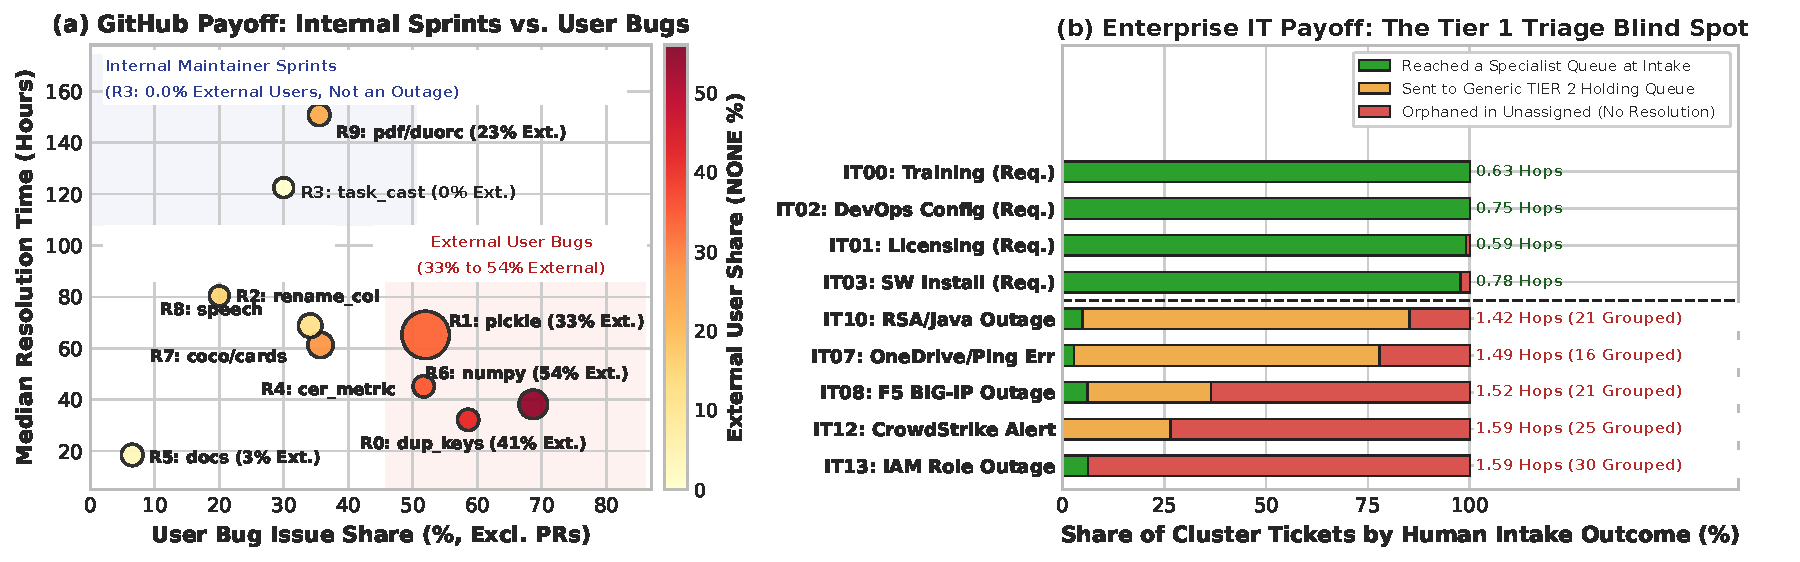
\includegraphics[width=0.92\textwidth]{figures/v3_figure5_payoff_triage.pdf}
  \caption{Extrinsic Validation Against GitHub Contributor Roles and Enterprise IT Intake Queues}
  \label{fig:extrinsic_mttr}
  \Description{Two panel figure showing (a) GitHub clusters placed by user bug issue share and median resolution time, colored by external user percentage, with shaded areas for the internal sprint cluster R3 and the external user bug clusters, and (b) Enterprise IT human intake outcome bars contrasting routine requests against cross boundary outages.}
\end{figure*}

The second failure mode of static two period monitoring, pooling cancellation, appears clearly in the enterprise IT stream~\cite{vogel2024itsm} (Figure~\ref{fig:temporal_sens}). When January baseline traffic ($N = 487$) is compared against pooled February and March traffic ($N = 851$), zero out of 14 clusters survive FDR control ($q \ge 0.23$), making the service desk appear completely stationary.

\begin{table}[!htbp]
  \caption{Coarse Versus Monthly Prevalence Shift Diagnostics on the Enterprise IT Stream}
  \label{tab:exp8}
  \footnotesize
  \setlength{\tabcolsep}{2.4pt}
  \begin{tabular}{llrrrr}
    \toprule
    ID & Subsystem & Coarse $\Delta$ & Mar $\Delta$ (95\% CI) & Mar $q$ & $\tau_{\text{MK}}$ \\
    \midrule
    IT03 & Installation & $-0.15$ (.94) & $\hl{+7.65}$ ($+3.0, +12.3$) & $\hl{.007}$ & $\hl{+.17}$ \\
    IT05 & File Crash & $+0.84$ (.90) & $+2.91$ ($-0.9, +6.8$) & $.231$ & $+.26$ \\
    IT02 & DevOps Config & $+1.06$ (.69) & $\hl{+2.81}$ ($+0.9, +4.8$) & $\hl{.007}$ & $\hl{+.46}$ \\
    IT04 & Report Export & $+0.53$ (.88) & $+1.58$ ($-0.2, +3.4$) & $.112$ & $+.28$ \\
    IT01 & Licensing & $-0.31$ (.94) & $+1.40$ ($-2.0, +4.8$) & $.469$ & $+.20$ \\
    IT08 & F5 BIG-IP Err & $-0.64$ (.88) & $\hl{-2.65}$ ($-4.1, -1.2$) & $\hl{.013}$ & $\hl{-.25}$ \\
    IT07 & OneDrive Err & $-3.16$ (.23) & $-2.92$ ($-5.4, -0.4$) & $.112$ & $-.19$ \\
    IT10 & RSA/Java Err & $-2.36$ (.69) & $\hl{-4.52}$ ($-7.9, -1.1$) & $\hl{.059}$ & $\hl{-.27}$ \\
    \bottomrule
  \end{tabular}
\end{table}

Panel a of Figure~\ref{fig:temporal_sens} shows why coarse pooling failed: in Software Installations (\texttt{IT03}), a February lull ($-4.43$ pp, dropping to $11.6\%$) and a March surge ($+9.88$ pp, rising to $21.5\%$) moved in opposite directions, pooling to $15.9\%$ and cancelling $99\%$ of their cumulative monthly variation when averaged together (Coarse $\Delta = -0.15$ pp, with BH FDR $q$ shown in parentheses in Table~\ref{tab:exp8}). Applying the monthly rule fixes this. February tested against January shows no significant shift ($q \ge 0.36$ for all 14 clusters), but March tested against January and February together reveals four significant shifts (Panel b of Figure~\ref{fig:temporal_sens} and Table~\ref{tab:exp8}), and the 14 day rolling trends ($\tau_{\text{MK}}$) point the same way: F5 BIG-IP load balancer errors (\texttt{IT08}) and RSA SecurID token errors (\texttt{IT10}) fell, while software installations (\texttt{IT03}) and department specific DevOps configurations (\texttt{IT02}) rose.

\section{The Payoff: Exposing Sprint False Alarms and Grouping Orphaned Tickets}

\subsection{GitHub Payoff: Cluster R3 Was an Internal Developer Sprint}
To verify that discovered clusters reflect genuine engineering workflows rather than lexical artifacts~\cite{hoyle2021automated, chen2020incidental}, we evaluate \texttt{R0} to \texttt{R9} against withheld GitHub metadata in Panel a of Figure~\ref{fig:extrinsic_mttr}: Pull Request versus user bug issue share, external community user share (\texttt{Ext.\%}, where \texttt{author\_association == NONE} rather than internal \texttt{MEMBER} or \texttt{CONTRIBUTOR}), and MTTR.

The withheld contributor roles in Panel a of Figure~\ref{fig:extrinsic_mttr} confirm our trajectory analysis. \textbf{0.0\% of records in \texttt{R3} (\texttt{task\_cast}) were submitted by external community users ($75\%$ core \texttt{MEMBER}, $25\%$ \texttt{CONTRIBUTOR})}, showing that the late May spike in Figure~\ref{fig:q2excess} was a coordinated internal refactoring sprint rather than a user outage. By contrast, the clusters behind the chronic and declining shifts (multiprocessing pickle crashes in \texttt{R1}, shard key hash collisions in \texttt{R0}, and NumPy and C++ wheel build failures in \texttt{R6}) draw $33\%$ to $54\%$ of their records from external users, the profile expected of genuine user bug outbreaks. Self contained documentation fixes sit at the other extreme (\texttt{R5}: $93.5\%$ PRs, $3\%$ external, $18.5$ h median MTTR).

\subsection{Enterprise IT Payoff: Grouping Orphaned Tickets from the Tier 1 Blind Spot}
\label{sec:ittriage}
On the enterprise service desk corpus~\cite{agarwal2012identifying, vogel2024itsm}, Panel b of Figure~\ref{fig:extrinsic_mttr} shows where the 314 orphaned \texttt{Unassigned} incidents sit. Routine service requests in the top four bars of Panel b (\texttt{IT00} to \texttt{IT03}) map unambiguously at intake to dedicated fulfillment queues (\texttt{Asset \& Vendor}, \texttt{SW Dev \& DevOps}, \texttt{End User Computing}), experiencing minimal reassignments ($0.59$ to $0.78$ hops) and virtually zero generic Tier 2 escalation or unassigned abandonment.

Conversely, across the five critical security, network, and identity outage clusters in the bottom bars of Panel b (\texttt{IT10}, \texttt{IT07}, \texttt{IT08}, \texttt{IT12}, and \texttt{IT13}), $93.8\%$ to $100\%$ of incoming tickets fail to reach a specialist team at Tier 1 intake, bouncing across repeated reassignments ($1.42$ to $1.59$ mean hops)~\cite{agarwal2012identifying, chen2020incidental}. Panel b of Figure~\ref{fig:extrinsic_mttr} shows two patterns: for authentication and cloud sync faults (\texttt{IT10} RSA/Java login tokens and \texttt{IT07} OneDrive/Ping single sign on), $75.0\%$ to $80.3\%$ of tickets land in the generic \texttt{TIER 2 TEAM} holding queue, whereas for infrastructure, endpoint security, and cloud permission faults (\texttt{IT08} F5 BIG-IP network load balancers, \texttt{IT12} CrowdStrike Falcon endpoint sensors, and \texttt{IT13} Identity and Access Management [IAM] roles), $63.6\%$ to $93.8\%$ of tickets remain orphaned in \texttt{Unassigned}. Grouping these contacts by their technical failure signatures (\texttt{f5 big ip}, \texttt{crowdstrike falcon}, \texttt{rsa token}, \texttt{ping identity}) isolates all five outage families and groups $237$ of the $314$ orphaned \texttt{Unassigned} incidents ($75.5\%$) with similar tickets that a team already handled, while leaving the $77$ ambiguous noise residuals in $C_{-1}$ for human review. This shows which queue each orphaned ticket resembles; it does not check that the queue would have resolved the ticket.

\section{Limitations}
Our study covers one open source repository and one enterprise benchmark, and the enterprise tickets are synthetic, so results on real helpdesks and other organizations may differ. Hyperparameters such as the $120$ ticket cap ($\sim\!14\%$ of SWE volume) and $14$ day rolling window were calibrated for streams arriving at $\sim\!5$ to $15$ tickets/day and must be scaled with arrival rate on much smaller or larger deployments. Several clusters are small (for example, \texttt{R3} has 20 tickets), GitHub \texttt{author\_association} roles are only a proxy for whether a contributor is internal, and fitting online without full period refitting is left for future work.

\section{Conclusion}
Turning unstructured ticket streams into reliable operational intelligence requires overcoming the lexical and temporal traps that distort standard topic models. Across open source and enterprise benchmarks, we showed that: (1) sliding window coherence ($C_v$) is inflated by ticket templates, whereas domain pruned c-TF-IDF and Bounded EOM on a 5D UMAP manifold split overmerged mega clusters into specific subsystems with $98.3\%$ type purity and $82.3\%$ subcategory purity; (2) pairing BH FDR tests with 14 day rolling windows at several time scales avoids pooling cancellation and separates chronic plateaus from internal maintainer sprints; and (3) checking clusters against withheld metadata exposes \texttt{R3} as an internal maintainer sprint and groups $75.5\%$ of orphaned incidents with similar tickets that a team already handled.

\bibliographystyle{ACM-Reference-Format}
\bibliography{references}

\end{document}
